% Options for packages loaded elsewhere
\PassOptionsToPackage{unicode}{hyperref}
\PassOptionsToPackage{hyphens}{url}
%
\documentclass[
  11pt]{scrartcl}
\usepackage{lmodern}
\usepackage{amssymb,amsmath}
\usepackage{ifxetex,ifluatex}
\ifnum 0\ifxetex 1\fi\ifluatex 1\fi=0 % if pdftex
  \usepackage[T1]{fontenc}
  \usepackage[utf8]{inputenc}
  \usepackage{textcomp} % provide euro and other symbols
\else % if luatex or xetex
  \usepackage{unicode-math}
  \defaultfontfeatures{Scale=MatchLowercase}
  \defaultfontfeatures[\rmfamily]{Ligatures=TeX,Scale=1}
\fi
% Use upquote if available, for straight quotes in verbatim environments
\IfFileExists{upquote.sty}{\usepackage{upquote}}{}
\IfFileExists{microtype.sty}{% use microtype if available
  \usepackage[]{microtype}
  \UseMicrotypeSet[protrusion]{basicmath} % disable protrusion for tt fonts
}{}
\makeatletter
\@ifundefined{KOMAClassName}{% if non-KOMA class
  \IfFileExists{parskip.sty}{%
    \usepackage{parskip}
  }{% else
    \setlength{\parindent}{0pt}
    \setlength{\parskip}{6pt plus 2pt minus 1pt}}
}{% if KOMA class
  \KOMAoptions{parskip=half}}
\makeatother
\usepackage{xcolor}
\IfFileExists{xurl.sty}{\usepackage{xurl}}{} % add URL line breaks if available
\IfFileExists{bookmark.sty}{\usepackage{bookmark}}{\usepackage{hyperref}}
\hypersetup{
  pdftitle={ manual},
  hidelinks,
  pdfcreator={LaTeX via pandoc}}
\urlstyle{same} % disable monospaced font for URLs
\usepackage[top=2.4cm,bottom=2.4cm,left=3.2cm,right=3cm,footskip=0.8cm]{geometry}
\usepackage{longtable,booktabs}
% Correct order of tables after \paragraph or \subparagraph
\usepackage{etoolbox}
\makeatletter
\patchcmd\longtable{\par}{\if@noskipsec\mbox{}\fi\par}{}{}
\makeatother
% Allow footnotes in longtable head/foot
\IfFileExists{footnotehyper.sty}{\usepackage{footnotehyper}}{\usepackage{footnote}}
\makesavenoteenv{longtable}
\usepackage{graphicx}
\makeatletter
\def\maxwidth{\ifdim\Gin@nat@width>\linewidth\linewidth\else\Gin@nat@width\fi}
\def\maxheight{\ifdim\Gin@nat@height>\textheight\textheight\else\Gin@nat@height\fi}
\makeatother
% Scale images if necessary, so that they will not overflow the page
% margins by default, and it is still possible to overwrite the defaults
% using explicit options in \includegraphics[width, height, ...]{}
\setkeys{Gin}{width=\maxwidth,height=\maxheight,keepaspectratio}
% Set default figure placement to htbp
\makeatletter
\def\fps@figure{htbp}
\makeatother
\setlength{\emergencystretch}{3em} % prevent overfull lines
\providecommand{\tightlist}{%
  \setlength{\itemsep}{0pt}\setlength{\parskip}{0pt}}
\setcounter{secnumdepth}{-\maxdimen} % remove section numbering
\usepackage{siunitx}
\usepackage[auth-sc]{authblk}
   \author[1]{Thomas Becher}
   \author[2]{Tobias Neumann}
   \affil[1]{Universität Bern, \url{becher@itp.unibe.ch}}
   \affil[2]{Brookhaven National Laboratory, \url{tneumann@bnl.gov}}
\ifluatex
  \usepackage{selnolig}  % disable illegal ligatures
\fi


\usepackage{scalefnt}
\newcommand{\abbrev}{\scalefont{.9}}

\newcommand{\NNLO}{\text{\abbrev NNLO}}




\title{
\includegraphics[width=2.08333in,height=\textheight]{figs/logo.pdf}
manual}
\date{MCFM v10.0, CuTe-MCFM v1.0 \\ updated March 2021}

\begin{document}
\maketitle
\begin{abstract}
CuTe-MCFM is an extension of MCFM for $q_T$ resummation and reaches N$^3$LL precision for all color-singlet processes included in MCFM at NNLO  ($W^\pm, Z, H$, $\gamma\gamma, Z\gamma, ZH, W^\pm H$). We document here the resummation features and refer the reader to the the MCFM manual (manual.pdf) for information on MCFM itself.
\end{abstract}

\tableofcontents

\hrulefill

This manual describes the installation, use and options for running CuTe-MCFM.
For a description of the resummation formalism, underlying choices, and
physics examples we refer to our publication \textit{JHEP 03 (2021) 199},
\href{https://arxiv.org/abs/2009.11437}{arXiv:2009.11437}. While the code is
easy to run, some parameters must be properly chosen to obtain sensible results. These include a technical cutoff on the matching corrections at low $q_T$ and the choice of a function which governs the transition from resummation to the fixed-order result. We will provide the definition of the parameters in this manual, and the appropriate choice for different processes is detailed in our publication.

\hypertarget{processes-available-for-resummation}{%
\subsection{Processes available for
resummation}\label{processes-available-for-resummation}}


The processes listed below are available for
N\(^3\)LL+NNLO computations. They can be calculated with or without decays.
Any further color-singlet processes implemented in MCFM at NNLO (NLO)
can easily be interfaced with N\(^3\)LL (N\(^2\)LL) \(q_T\)
resummation.\footnote{We are happy to provide
    details about how to do this.}

The first set of processes below have been thoroughly studied as part of our
publication. We provide input files with a suitably chosen set of input
parameters for all of them.

\begin{itemize}
\tightlist
\item
  \(W^+(\to e^+ \nu)\) (\texttt{nproc=1}) (\texttt{input\_W+.ini})
\item
  \(W^-(\to e^- \bar\nu)\) (\texttt{nproc=6}) (\texttt{input\_W-.ini})
\item
  \(Z(\to e^+ e^-)\) (\texttt{nproc=31}) (\texttt{input\_Z.ini})
\item
  \(H(\to \gamma \gamma)\) (\texttt{nproc=119})
  (\texttt{input\_Higgs.ini})
\item
  \(\gamma\, \gamma\) (\texttt{nproc=285})
  (\texttt{input\_GammaGamma.ini})
\item
  \(gg \to \gamma\, \gamma\) at N\(^2\)LL+NLO (\texttt{nproc=2851})
\item
  \(Z(\to e^+ e^-)\, \gamma\) (\texttt{nproc=300})
  (\texttt{input\_ZGamma.ini})
\end{itemize}

The second set of processes below are ready to use, and we have checked that the
fixed-order expansion of the resummed result and the fixed-order
cross-section approach each other towards \(q_T\to0\). However, the transition
function parameter might need adjustment. Please contact the
authors if you are unsure about this.

\(Z\) production:

\begin{itemize}
\tightlist
\item
  \(Z(\to 3\nu \bar\nu)\) (\texttt{nproc=32})
\end{itemize}

Higgs production:

\begin{itemize}
\tightlist
\item
  \(H(\to \tau \bar\tau)\) (\texttt{nproc=112})
\item
  \(H(\to b \bar b)\) (\texttt{nproc=111})
\end{itemize}

\(Z\gamma\) production:

\begin{itemize}
\tightlist
\item
  \(Z(\to 3 \nu \bar\nu)\, \gamma\) (\texttt{nproc=305})
\end{itemize}

\(W^\pm H\) production:

\begin{itemize}
\tightlist
\item
  \(W^+(\to e^+ \nu )\, H(\to \tau \bar\tau)\) (\texttt{nproc=91})
\item
  \(W^+(\to e^+ \nu )\, H(\to b \bar b)\) (\texttt{nproc=92})
\item
  \(W^-(\to e^- \bar\nu )\, H(\to \tau \bar\tau)\) (\texttt{nproc=96})
\item
  \(W^-(\to e^- \bar\nu )\, H(\to b \bar b)\) (\texttt{nproc=97})
\item
  \(W^+(\to e^+ \nu )\, H(\to \gamma\gamma)\) (\texttt{nproc=93})
\item
  \(W^-(\to e^- \bar\nu )\, H(\to \gamma\gamma)\) (\texttt{nproc=98})
\end{itemize}

\(ZH\) production:

\begin{itemize}
\tightlist
\item
  \(Z(\to e^+ e^-) \, H(\to \tau \bar\tau)\) (\texttt{nproc=110})
\item
  \(Z(\to e^+ e^-) \, H(\to b \bar b)\) (\texttt{nproc=101})
\item
  \(Z(\to e^+ e^-) \, H(\to \gamma \gamma)\) (\texttt{nproc=104})
\end{itemize}

Further decay channels are available in principle, but will need some
checking. Please contact the authors if you are interested in a specific process.

\hypertarget{mcfm-compilation-quick-start}{%
\subsection{MCFM compilation quick
start}\label{mcfm-compilation-quick-start}}

Please refer to the full MCFM manual for details beyond this quick start
guide. In the simplest case (on most Linux systems), to install CuTe-MCFM and
all dependencies for execution on a single computer, execute the command
\texttt{cmake ..} in the \texttt{Bin} directory.

MCFM requires the GNU compiler gcc/g++ and gfortran version 7 or greater.
Please type \texttt{gfortran --version} to verify the compiler version. On some systems
these commands are linked against a different compiler. For example on Mac OS X systems this is typically the case. To set the correct compiler commands please add the flags
\texttt{-DCMAKE\_Fortran\_COMPILER=mygfortran},
\texttt{-DCMAKE\_C\_COMPILER=mygcc} and
\texttt{-DCMAKE\_CXX\_COMPILER=myg++}, where \texttt{mygfortran},
\texttt{mygcc} and \texttt{myg++} are the commands for the Fortran, C,
and C++ compilers of the GNU gcc suite of at least version 7. That is,
in the \texttt{Bin} directory run cmake with the specified compiler commands as in
\texttt{cmake .. -DCMAKE\_Fortran\_Compiler=mygfortran}.


By default a bundled LHAPDF library is compiled and linked against. If you
prefer to use a system installation please add the cmake options
\texttt{-Duse\_internal\_lhapdf=Off -Duse\_external\_lhapdf=On}.\footnote{Do
not use an external installation of version LHAPDF-6.3.0 or newer, since this
has a critical multithreading bug.} If the library is in a non-standard
location another option like \texttt{-DCMAKE\_PREFIX\_PATH=/usr/local}, which
adds the path to the cmake library search path, might be necessary.

If CMake does not report any problems you can start the compilation of
MCFM with \texttt{make -j4}, where 4 (or more) is the number of
compilation threads.

Upon successful compilation, the executable \texttt{mcfm} is produced and
can be called with an input file as argument, for example \texttt{./mcfm input\_Z.ini}.

To prepare MCFM with MPI
support add the argument \texttt{-Duse\_mpi=On} to the cmake call before
running \text{make}. At the same time custom compiler command names must
be specified with \texttt{-DCMAKE\_Fortran\_COMPILER=mpifort} and
\texttt{-DCMAKE\_CXX\_COMPILER=mpic++}. The commands \texttt{mpifort}
and \texttt{mpic++} must be used when compiling with MPI support. In
this case, please ensure again that \texttt{mpifort ----version} and
\texttt{mpic++ ----version} report the GNU compiler and a version
greater than 7.

It can happen that the CMake cache gets corrupted with wrong
configuration options. If you change options and errors occur, please
try to delete the file \texttt{CMakeCache.txt} and directory
\texttt{CMakeFiles} and restart \texttt{cmake ..} with the appropriate arguments.

\hypertarget{using-cute-mcfm-resummation}{%
\subsection{Using CuTe-MCFM
resummation}\label{using-cute-mcfm-resummation}}

While CuTe-MCFM can calculate \(q_T\)-resummed results without using
pregenerated beam functions grids, we recommend that LHAPDF grid files are
generated for the beam functions beforehand for a choice of a PDF set. This
\emph{significantly} accelerates the evaluation of the beam functions and the
integration.

CuTe-MCFM ships with pregenerated beamfunction grids for the central
values of \texttt{CT14nnlo} and \texttt{NNPDF31\_nnlo\_as\_0118}, which
are included in the \texttt{Bin/PDFs} directory. This path is automatically used
as the preferred path for LHAPDF grid files. With these pregenerated
grids the example input files work out of the box. For other PDF sets or
when using PDF errors, the first run of CuTe-MCFM should be with the
setting \texttt{makegrid=.true.}. Additionally the input and output
directories for the PDF grids have to be specified. For example the
input directory is typically \texttt{/usr/local/share/LHAPDF/} (or the
\texttt{PDFs/} directory relative to the mcfm executable in \texttt{Bin}) and
the output directory should be a user-writeable directory like
\texttt{/home/user/gridout/} (or \texttt{PDFs/}). Note the trailing slashes.

When calling mcfm with \texttt{makegrid=.true.} only the beam function
grids are written during that run, and mcfm exits afterwards.
We recommend to use \texttt{PDFs/} as the gridout path, since this
path is automatically added to the LHAPDF search paths, and you won't have to
copy the generated grid directories to your LHAPDF grid directory or set the
\texttt{LHAPDF\_DATA\_PATH} environment variable to the gridout path.

For example for the set CT14nnlo the grid directories
\texttt{CT14nnlo\_B00}, \texttt{CT14nnlo\_B10}, \texttt{CT14nnlo\_B11},
\texttt{CT14nnlo\_B20}, \texttt{CT14nnlo\_B21}, \texttt{CT14nnlo\_B22} and \texttt{CT14nnlo\_G10} are written and have to be copied to the
directory where LHAPDF searches for the grid files. When the gridout path is chosen as \texttt{PDFs/} no further action is necessary. The LHAPDF grid file
search path can be modified by setting the shell
environment variable \texttt{LHAPDF\_DATA\_PATH} to the desired
directory, but the \texttt{PDFs} directory is always used as the preferred directory.


The next run of mcfm should be done with \texttt{makegrid=.false.} and
\texttt{usegrid=.true.}.

Other important parameters for the resummation are \texttt{res\_range},
determining the integration range of the purely resummed part,
\texttt{resexp\_range}, determining the integration range of the
fixed-order expanded resummed part, and \texttt{fo\_cutoff} which sets
the lower \(q_T\) cutoff for the fixed-order part. Typically this cutoff
should agree with the lower range of \texttt{resexp\_range}. For example
for \(Z\) production one can integrate up to \(m_Z\) with a cutoff of
\SI{1}{\GeV}: \texttt{res\_range = 0.0 90.0},
\texttt{resexp\_range = 1.0 90.0}, \texttt{qt\_cutoff = 1.0}.

For details regarding these parameters see the next section. The
transition function is also discussed below.

\hypertarget{input-file-parameters}{%
\subsection{Input file parameters}\label{input-file-parameters}}

The \texttt{[resummation]} section has been added to the input file to
control the resummation. The following keys are available:

\begin{longtable}[]{@{}ll@{}}
\toprule
\begin{minipage}[b]{0.24\columnwidth}\raggedright
Key\strut
\end{minipage} & \begin{minipage}[b]{0.71\columnwidth}\raggedright
Description\strut
\end{minipage}\tabularnewline
\midrule
\endhead
\begin{minipage}[t]{0.24\columnwidth}\raggedright
\texttt{usegrid}\strut
\end{minipage} & \begin{minipage}[t]{0.71\columnwidth}\raggedright
\texttt{.true.} or \texttt{.false.} determines whether pregenerated
LHAPDF interpolation grids should be used for the resummation beam
functions.\strut
\end{minipage}\tabularnewline
\begin{minipage}[t]{0.24\columnwidth}\raggedright
\texttt{makegrid}\strut
\end{minipage} & \begin{minipage}[t]{0.71\columnwidth}\raggedright
If \texttt{.true.}, then MCFM runs in grid generation mode. This
generates LHAPDF grid files in the directory \texttt{gridoutpath} from
LHAPDF grids in the directory \texttt{gridinpath}. After the grid
generation MCFM stops and should be run subsequently with
\texttt{makegrid = .false.} and \texttt{usegrid = .true.}. When
\texttt{lhapdf\%dopdferrors=.true.} then also grids for the error sets
are generated.\strut
\end{minipage}\tabularnewline
\begin{minipage}[t]{0.24\columnwidth}\raggedright
\texttt{gridoutpath}\strut
\end{minipage} & \begin{minipage}[t]{0.71\columnwidth}\raggedright
Output directory for LHAPDF grid files, for example
\texttt{/home/tobias/local/share/LHAPDF/}\strut
\end{minipage}\tabularnewline
\begin{minipage}[t]{0.24\columnwidth}\raggedright
\texttt{gridinpath}\strut
\end{minipage} & \begin{minipage}[t]{0.71\columnwidth}\raggedright
Input directory for LHAPDF grid files, for example
\texttt{/home/tobias/local/share/LHAPDF/}\strut
\end{minipage}\tabularnewline
\begin{minipage}[t]{0.24\columnwidth}\raggedright
\texttt{res\_range}\strut
\end{minipage} & \begin{minipage}[t]{0.71\columnwidth}\raggedright
Integration range of purely resummed part, for example \texttt{0.0 80.0}
for \(q_T\) integration between 0 and 80 GeV.\strut
\end{minipage}\tabularnewline
\begin{minipage}[t]{0.24\columnwidth}\raggedright
\texttt{resexp\_range}\strut
\end{minipage} & \begin{minipage}[t]{0.71\columnwidth}\raggedright
Integration range of fixed-order expanded resummed part, for example
\texttt{1.0 80.0} for \(q_T\) integration between 1 and 80 GeV.\strut
\end{minipage}\tabularnewline
\begin{minipage}[t]{0.24\columnwidth}\raggedright
\texttt{fo\_cutoff}\strut
\end{minipage} & \begin{minipage}[t]{0.71\columnwidth}\raggedright
Lower \(q_T\) cutoff $q_0$ for the fixed-order part, see eq.~\eqref{eq:matchingmod} below. Typically the value should agree with the lower range of \texttt{resexp\_range}.\strut
\end{minipage}\tabularnewline
\begin{minipage}[t]{0.24\columnwidth}\raggedright
\texttt{transitionswitch}\strut
\end{minipage} & \begin{minipage}[t]{0.71\columnwidth}\raggedright
Parameter passed to the plotting routine to modify the transition
function, see text.\strut
\end{minipage}\tabularnewline
\bottomrule
\end{longtable}

We strongly recommend to calculate resummed results with pregenerated
grids, see the previous section.
The integration range for the purely resummed part can be controlled with the key
\texttt{res\_range} and should typically be between \(0\) and some upper
value. For example for \(W^\pm, Z\) or \(H\) production this can just be
the boson mass. For other processes there can be thresholds and this
number must be selected more carefully to not run into numerical issues,
see arXiv:2009.11437.

The setting \texttt{resexp\_range} and \texttt{fo\_cutoff} are relevant
for the matching corrections. The values of the \texttt{resexp\_range}
determine the integration range for the fixed-order expansion of the
resummed part. The minimum should typically be at least one GeV for
numerical stability. For smaller values significantly more time goes
into the integration, and the minimum number of Vegas calls might need
to increased. For single boson processes the maximum value can again be
the boson mass, although it can be set to a value where the implemented
transition function fully switches to zero. The fixed-order cutoff
\texttt{fo\_cutoff} determines the minimum \(q_T\) for the fixed-order
calculation. This should typically agree with the lower range of the
\texttt{resexp\_range}.

Lastly, the parameter \texttt{transitionswitch} is passed for
convenience to the plotting routines where the transition function is
implemented. It can be used for for an easy control of the transition
region as described in the following.

\hypertarget{plotting-and-transition}{%
\subsection{Plotting routine and transition function}\label{plotting-and-transition}}

The following transition function is implemented for the example
input files. For more details we refer to our publication. The fully
matched cross-section is described in general by 
\begin{equation}\label{eq:matchingmod}
\left.\frac{\mathrm{d}\sigma^{\text{N$^3$LL}}}{\mathrm{d}q_T}\right|_\text{matched to \NNLO{}} 
=  t(x) \left( \frac{\mathrm{d}\sigma^{\text{N$^3$LL}}}{\mathrm{d}q_T} + 
\left.\Delta\sigma\right|_{q_T>q_0} \right)
+ (1-t(x)) \frac{\mathrm{d}\sigma^\NNLO{}}{\mathrm{d}q_T}\,
\end{equation}
using a transition function $t(x)$. We have implemented a transition function $t$
with $x=q_T^2/Q^2$ that smoothly switches between 1 and 0 like a sigmoid function.

Following a choice in CuTe, we first define
\[
s(x;l,r,u) = \left (1 + \exp\left(\log\left(\frac{1-u}{u}\right) \frac{x-m}{w}\right) \right 
)^{-1}\,,\quad
m = (r+l)/2\,,\quad w = (r-l)/2\,.
\]
The function $s(x)$, parametrized by $l,r,u$, is defined to be $s(l)=1-u$ and $s(r)=u$.
In terms of this sigmoid, our transition function $t(x; x^\text{min},x^\text{max},u)$, where $x=q_T^2/Q^2$, is then defined by
\begin{equation}\label{eq:transition}
t(x; x^\text{min},x^\text{max},u) = \left\{\begin{array}{lr}
1 , & \text{for } x < x^\text{min}\\
\frac{s(x; x^\text{min}, x^\text{max},u)}{s(x^\text{min}; x^\text{min}, x^\text{max},u)}, & 
\text{otherwise}
\end{array}\right\}\,.
\end{equation}
This ensures that below $x^\text{min}=(q_T^\text{min}/Q)^2$ only the naively matched result is 
used, and at
$x^\text{max}$
for small $u\ll1$ the transition function is approximately $u$. In practice it makes sense to set 
the transition
function to zero below a small threshold like $10^{-3}$ without a noticeable discontinuity.
This has the advantage that the deteriorating resummation and matching corrections do not impact 
the region of 
large $q_T$ at all.
Our example plotting routines use $x^\text{min}=0.001$, and $u=0.001$, and the parameter $x^\text{max}$ corresponds to the value of \texttt{transitionswitch} set in the input file. The transition function can be changed or completely replaced by just modifying the plotting routines. The following figure illustrates this transition function.

\begin{figure}[t!]
	\centering
	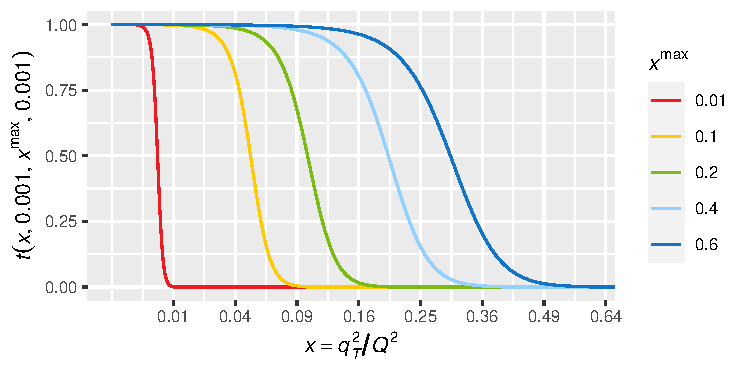
\includegraphics{figs/transition.pdf}
    \caption{The transition function defined in eq.~\eqref{eq:transition} for different values of the parameter $x^\text{max}$ which determines the position of the 
	transition. The $x$-axis is displayed on a square-root scale 
		to guide the eye on 
		the quadratic $q_T$-dependence.}
	\label{fig:transition}
\end{figure}

\paragraph{Modifying the plotting routines and transition function.}
The plotting infrastructure has been completely rewritten in this
version of MCFM, and we recommended to only use the new infrastructure
from this point on by setting \texttt{histogram\%newstyle = .true.} in
the input file. This is the default for the CuTe-MCFM example input files.

For the processes \(W^\pm,Z,H\), \(\gamma\gamma\), \(Z\gamma\), \(ZH\)
and \(W^\pm H\) we include predefined plotting routines that can be
adjusted. For example for \(Z\) production the plotting routine is in the file
\texttt{src/User/nplotter\_Z\_new.f90}, and similarly for the other processes.
The routine \texttt{setup} defines all histograms with custom or uniform
binning and names. The
number of used histograms needs to be allocated in this routine. The
routine \texttt{book} is called for each phase space point. Through the
boolean variable \texttt{abovecut} it is known whether the routine is
called for ``boosted \(q_T=0\)'' (resummed part and fixed-order expansion of
resummed part) or for \(q_T>0\) (fixed-order). All provided example input files
use the transition function as defined above, see also arXiv:2009.11437.

The plotting routine returns the calculated observables in the
\texttt{vals} array, and Vegas weights in \texttt{wts}. The transition
function is implemented by reweighting the original Vegas weights with
the output of the transition function. To disable the transition
function, one sets \texttt{trans} to \(1\) before filling the \texttt{wts}
array.

Apart from modifying a default set of kinematical cuts in the input
file, cuts can also be set in the file
\texttt{src/User/gencuts\_user.f90} in a fully flexible way based on the
event's four momenta. Some commented out examples are included there.

\hypertarget{development-details}{%
\section{Development details}\label{development-details}}

We briefly document information for modifying and extending the
resummation code.

\hypertarget{relevant-files-for-q_t-resummation}{%
\subsection{\texorpdfstring{Relevant files for \(q_T\)
resummation}{Relevant files for q\_T resummation}}\label{relevant-files-for-q_t-resummation}}

\begin{itemize}
\tightlist
\item
  \texttt{src/Mods/mod\_Beamfunctions.f90}: Implementation of beam
  functions. \texttt{getbeam} returns beam function components for a
  specified power of \(\alpha_s\) and \(L_\perp\) for \(q\bar{q}\)
  initial states, while \texttt{getbeam2} is for \(gg\) initial states.
\item
  \texttt{src/Mods/mod\_ResummationGrid.f90}: Implementation of LHAPDF
  grid generation for beam functions, with implementations for OpenMP,
  MPI and Fortran Coarrays.
\item
  \texttt{src/Mods/mod\_Resummation\_params.f90}: Saves integration
  range variables from input file.
\item
  \texttt{src/Mods/mod\_ResummationFourier.f90}: Implementation of
  Fourier integral for both \(q\bar{q}\) and \(gg\) initial states.
\item
  \texttt{src/Mods/mod\_Resummation.f90} Ties together all components
  above in subroutine \texttt{resummation}; determines scale \(q^*\);
  proper evolution of \(\alpha_s\) over quark mass thresholds; includes
  procedure for recoil boost;
\item
  \texttt{src/Procdep/resint.f90}: Overall integration routine that
  generates phase-space; calls boost routine; evaluates matrix elements;
  calls resummation and fixed-order expansion of resummation
\end{itemize}

\end{document}
